\documentclass[12pt, a4paper, hidelinks]{article}

\usepackage[icelandic]{babel}
\usepackage[T1]{fontenc}
\usepackage[utf8]{inputenc}


\usepackage{amsmath, amssymb, amsfonts}
\usepackage{mathtools}

\usepackage[outputdir=cache]{minted}
\usemintedstyle{default}
\renewcommand{\listingscaption}{Forrit}

\usepackage{url}
\usepackage{hyperref}
\usepackage[hang, flushmargin, bottom]{footmisc}

\usepackage[svgnames]{xcolor}
\usepackage{tabularx}
\usepackage{float}
\usepackage{graphicx}
\usepackage{booktabs}
\usepackage{enumerate}
\usepackage{multirow}
\usepackage{tikz}
\usepackage{tikz-qtree}
\usepackage{pifont}
\usepackage{multicol}
\usepackage{tcolorbox}
\usepackage{forest}

\newcommand{\cmark}{\color{Green}\ding{51}}
\newcommand{\xmark}{\color{Red}\ding{55}}

\usepackage{times, mathptmx}
\usepackage[scaled=0.85]{beramono}

\newenvironment{code}{\captionsetup{type=listing}}{}

\usepackage{fancyhdr}
\pagestyle{fancy}
\fancyhf{}
\fancyhead[L]{Kári Hlynsson}
\fancyhead[C]{TÖL203G HEIMADÆMI 5}
\fancyhead[R]{\today}
\fancyfoot[C]{\thepage}

\newcommand{\doctitle}{\uppercase{Heimadæmi 5}}
\newcommand{\coursename}{Tölvunarfræði 2}
\newcommand{\coursenum}{TÖL203G}

% ——— Mengjatákn
\newcommand{\N}{\mathbb{N}}
\newcommand{\Z}{\mathbb{Z}}
\newcommand{\Q}{\mathbb{Q}}
\newcommand{\R}{\mathbb{R}}
\newcommand{\C}{\mathbb{C}}

% ——— Vigrar
\renewcommand{\u}{\mathbf{u}}
\renewcommand{\v}{\mathbf{v}}
\renewcommand{\b}{\mathbf{b}}
\newcommand{\w}{\mathbf{w}}
\newcommand{\p}{\mathbf{p}}
\newcommand{\x}{\mathbf{x}}
\newcommand{\y}{\mathbf{y}}
\newcommand{\z}{\mathbf{z}}

% Define styles for nodes in the binary tree
\tikzset{
  binarytree/.style={
    draw,
    circle,
    thick,
    minimum size=0.75cm,
    inner sep=0pt,
    font=\sffamily\small
  },
  binaryedge/.style={
    draw,
    line width=1mm,
    red
  },
  binarytree empty/.style={
    draw=none,
    fill=none
  }
}

\begin{document}
\thispagestyle{plain}
\centerline{\bfseries\Large\doctitle}
\medskip
\centerline{\large\coursenum\ \coursename}
\bigskip

\centerline{\large Kári Hlynsson\footnote{Slóð á Github kóða: \url{https://github.com/lvthnn/TOL203G/tree/master/HD6}}}
\bigskip
\centerline{Háskóli Íslands}
\medskip
\centerline{\today}

\section*{Verkefni 1}
Þið eigið að breyta táknatöfluútfærslunni \texttt{SequentialSearchST.java}, þannig að
listinn sé sjálfskipandi (\emph{self-organizing}). Sjálfskipandi gagnagrindur laga sig
að notkunarmynstri notandans, þannig að lyklar sem oft er leitað að finnast hraðar en
þeir sem sjaldan er leitað að. Þið eigið að útfæra tiltekna útgáfu sem kallast færa-fremst
(\emph{move-to-front}). Hún felst í því að þegar kallað er á \texttt{get(k)}, þá er hnúturinn
með lyklinum \texttt{k} færður fremst í tengda listann (ef hann finnst). Það þýðir að ef leitað
er aftur að \texttt{k} fljótlega þá finnst hann hratt.

Þið eigið að skila breytta fallinu \text{get} og skjáskoti af keyrslu á \texttt{main}-fallinu fyrir
inntakið \texttt{A B R A C A D A B R A}, sem þið sláið inn eða pípið úr skrá. Útkoman ætti að vera
\texttt{D 6, C 4, R 9, B 8, A 10}, þ.e. sætisnúmerin á síðasta tilvikinu af hverjum staf.

\subsection*{Lausn}
\textsc{Forrit} \ref{forrit:faerafremst} á næstu síðu sýnir breyttu útfærsluna á \texttt{get} fallinu í \texttt{SequentialSearchST}
klasanum. Hugmyndin er sú að ef við finnum stakið sem við erum að leita ítrum við í gegnum tengda listann fram
að stakinu og skiptum á því og fyrsta stakinu í tengda listanum. Niðurstaðan er sú að við hliðrum öllum gildunum
frá hinu fyrsta fram til þess sem gildið sem var leitað að er í. Síðan er skipt á því og fyrsta stakinu sem er það
sem við viljum.

\textsc{Mynd 1} sýnir skjáskot af keyrslu.
\begin{listing}[H]
    \centering
    \inputminted[
        firstline=66, 
        lastline=86, 
        gobble=3, 
        frame=single,
        fontsize=\footnotesize,
        linenos,
        breaklines
        ]{java}{../src/V1/SequentialSearchST.java}
    \caption{Útfærsla á færa-fremst aðferð í \texttt{get} fallinu}
    \label{forrit:faerafremst}
\end{listing}
\begin{figure}[H]
   \centering
   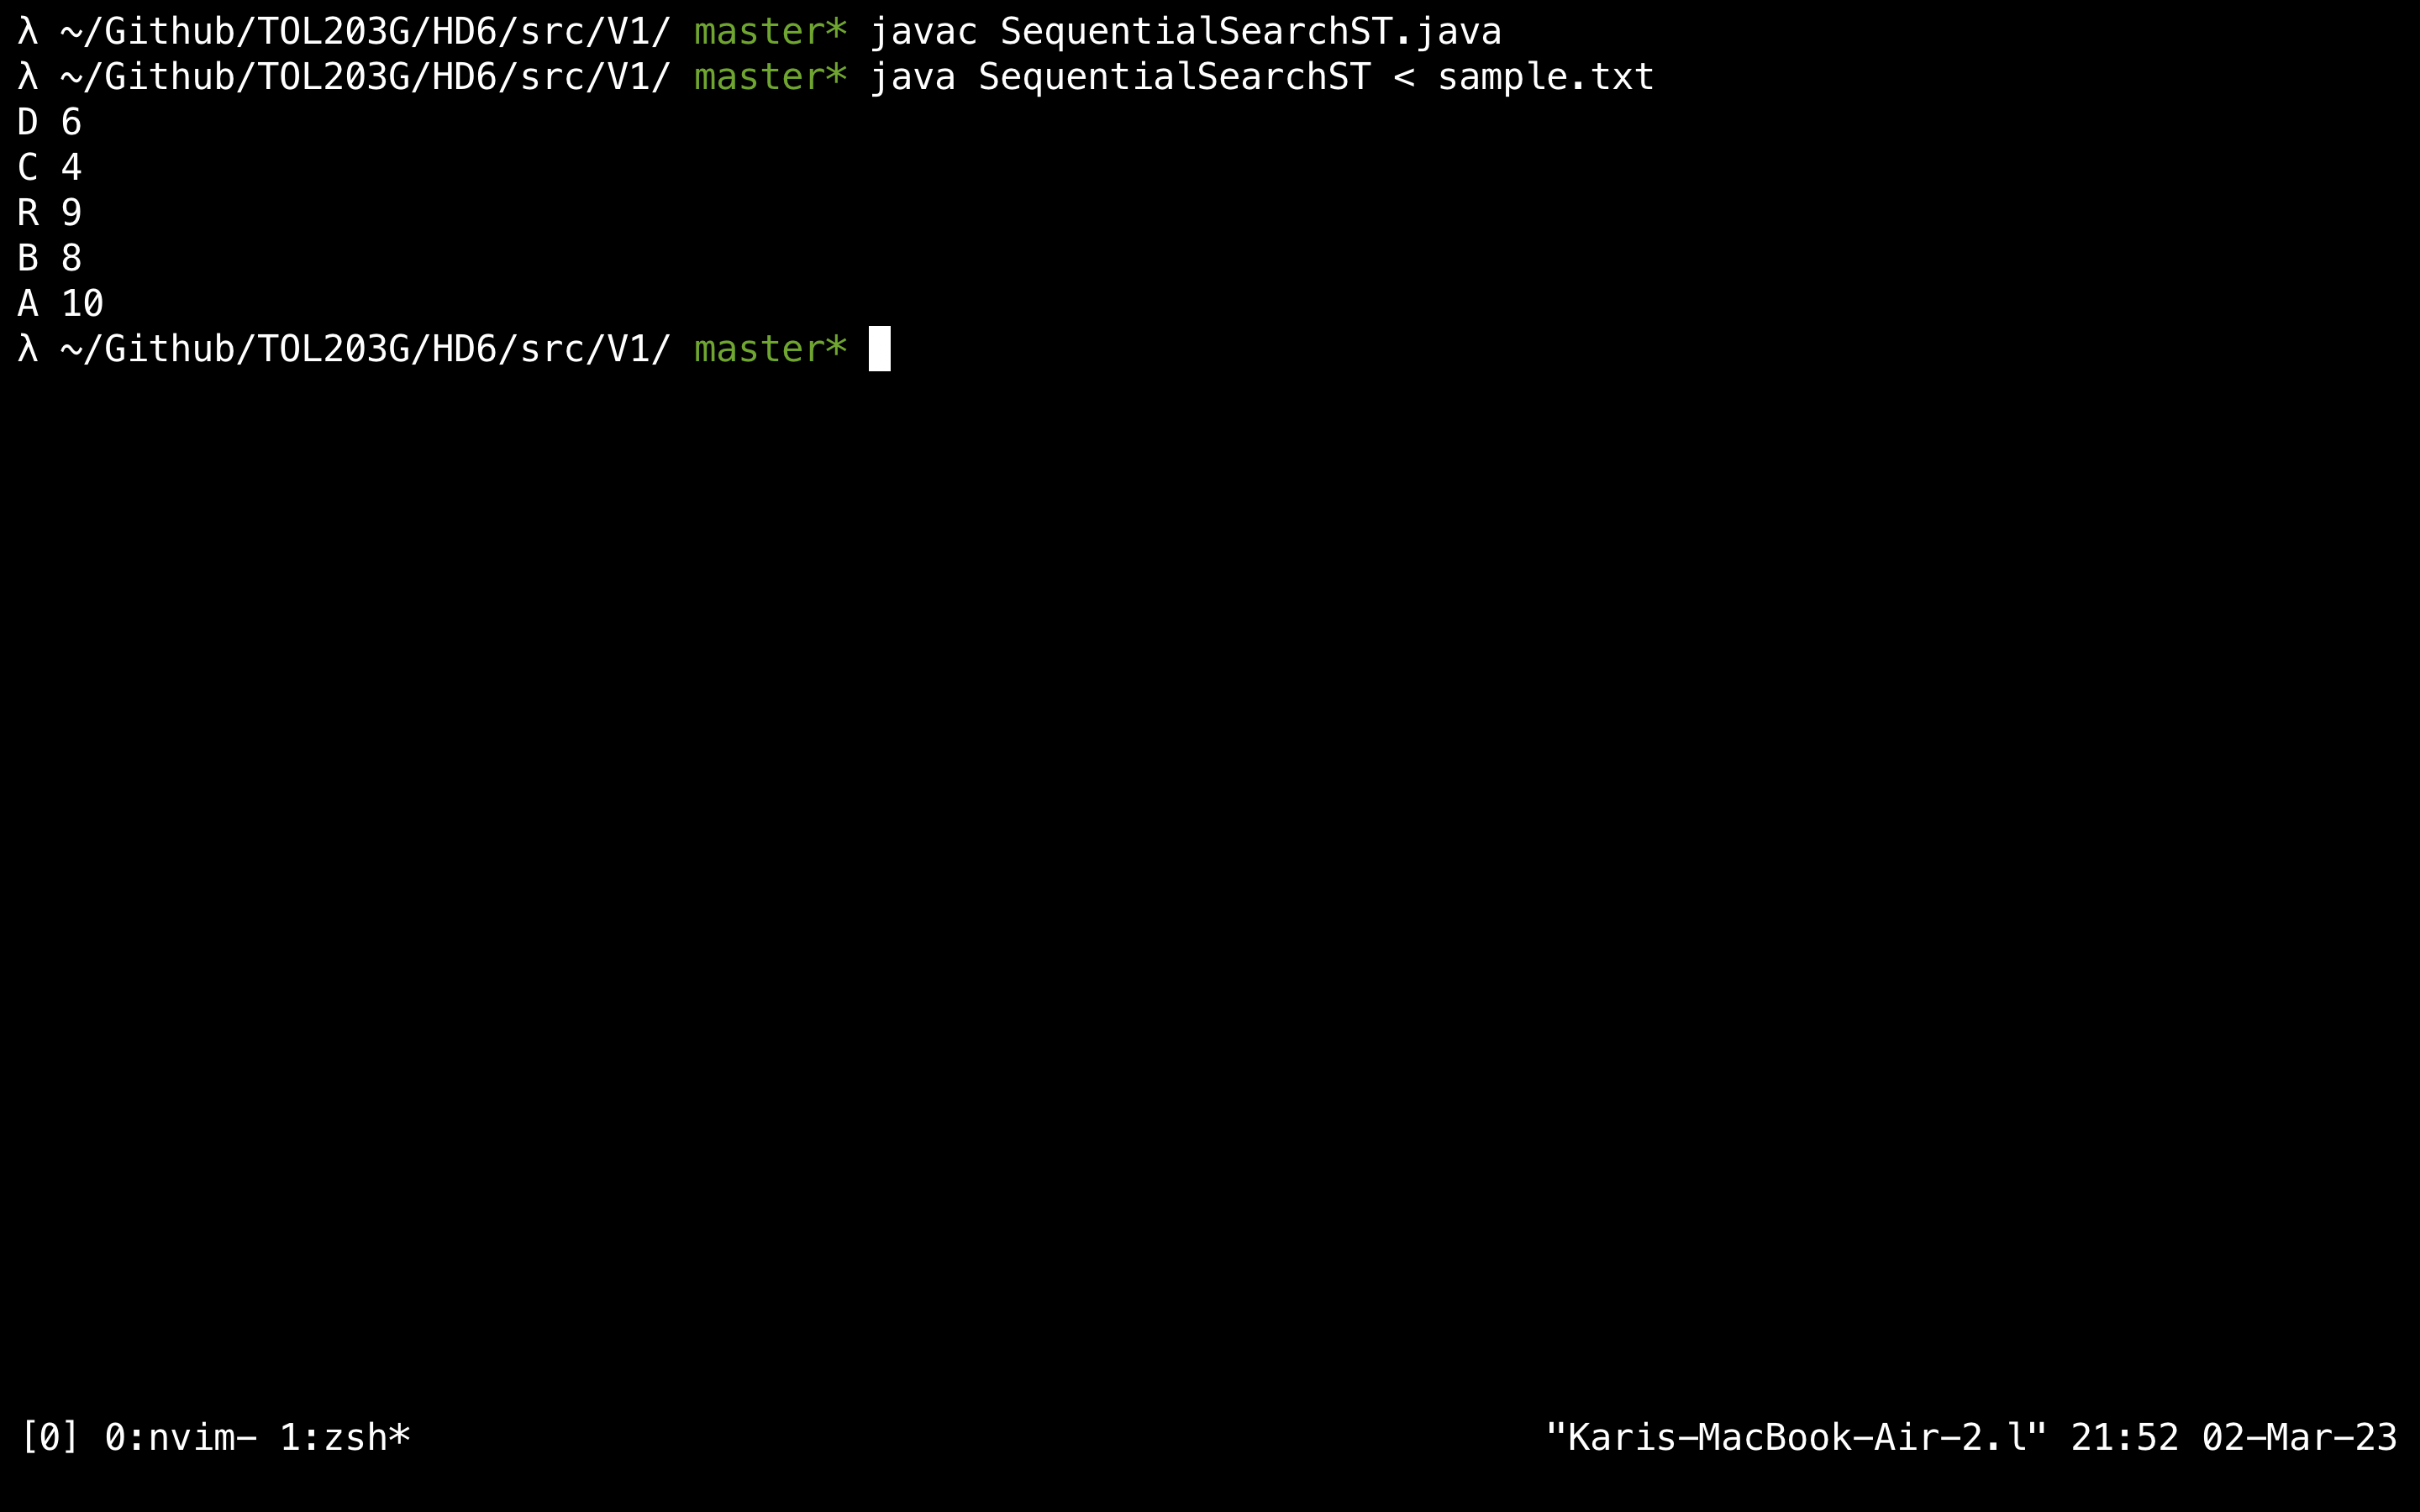
\includegraphics[width=\textwidth]{img/v1-keyrsla.png}
   \caption{Keyrsla á \texttt{SequentialSearchST.java} í skel}
\end{figure}

\newpage

\section*{Verkefni 2}
Dæmi 3.1.28 á bls. 392 í kennslubók. Það á að breyta fallinu \texttt{put} í klasanum
\texttt{BinarySearchST.java} þannig að ef nýr lykill er stærri en allir lyklarnir í töflunni
þá er hann settur inn í föstum (þ.e. $\Theta(1)$ í stað $\Theta(\log N)$). Skilið breytta fallinu
\texttt{put} og skjámynd af keyrslu á inntakinu \texttt{A B C D E F G H}.

\subsection*{Lausn}
\begin{listing}[H]
   \centering
   \inputminted[
    firstline=121, 
    lastline=153, 
    gobble=3, 
    frame=single,
    fontsize=\footnotesize,
    linenos,
    breaklines
   ]{java}{../src/V2/BinarySearchST.java} 
   \caption{Breytt útfærsla á \texttt{put} í \texttt{BinarySearchTree.java}}
\end{listing}

\newpage

\begin{figure}[H]
   \centering
   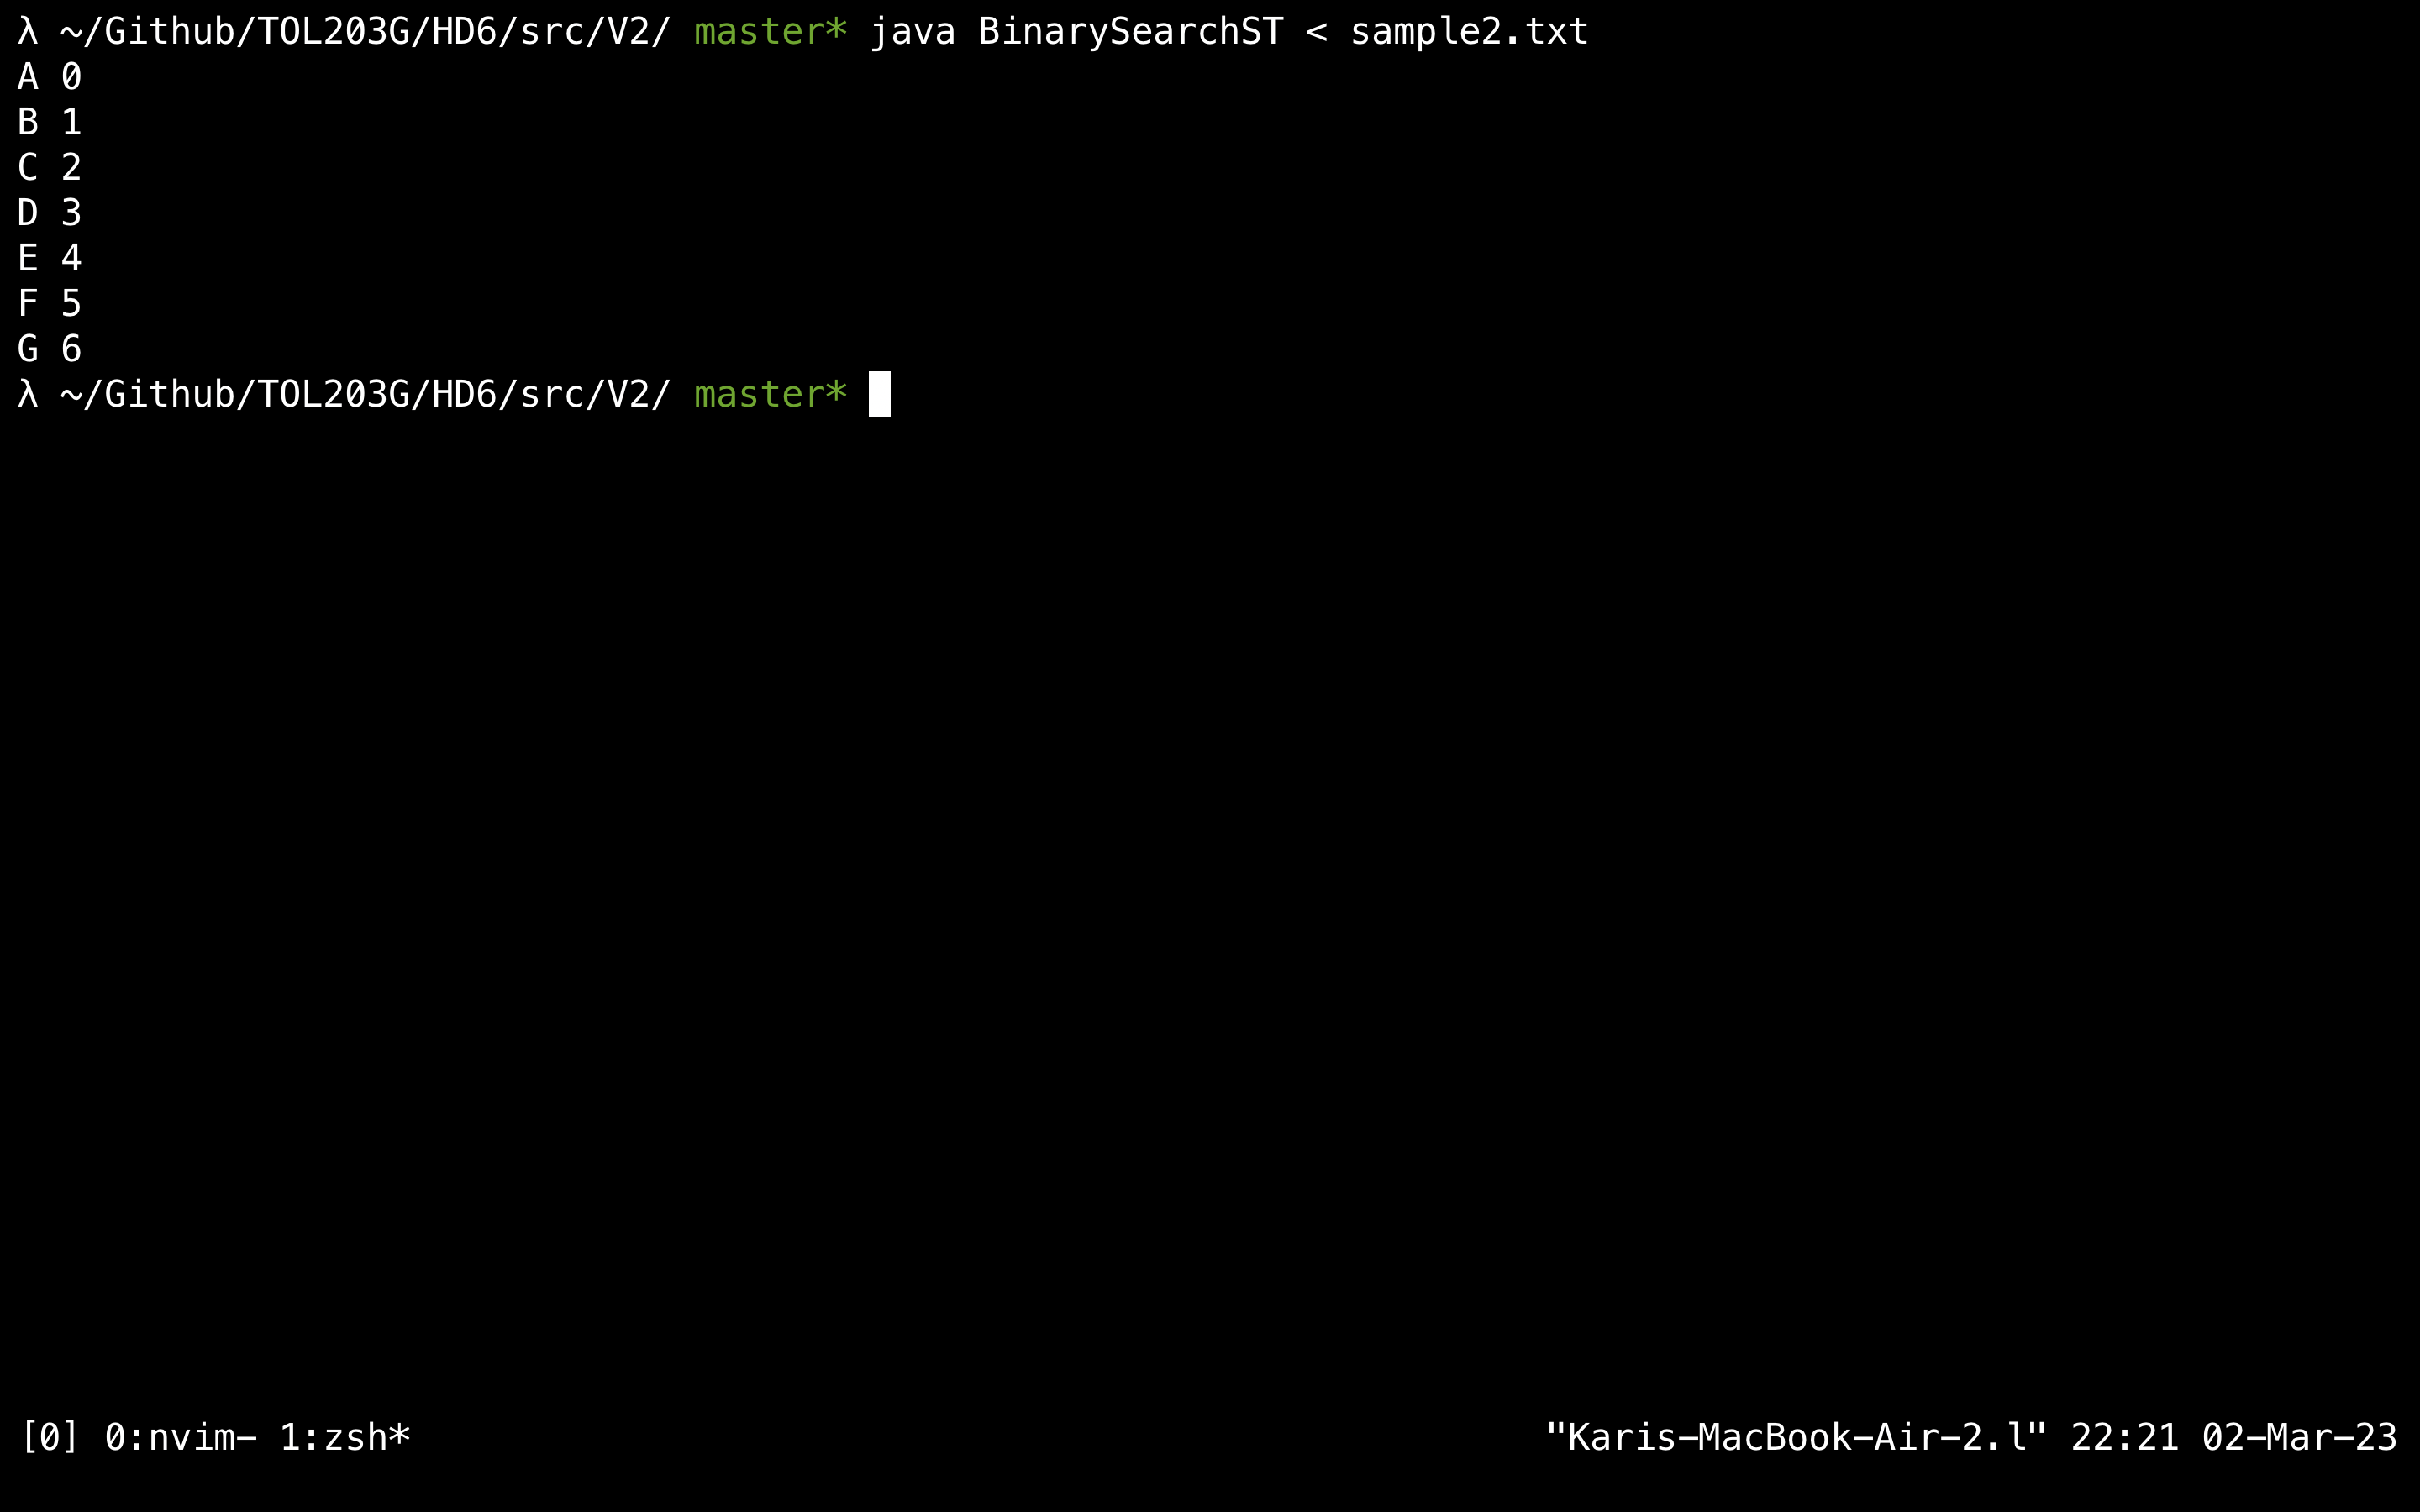
\includegraphics[width=\textwidth]{img/v2-keyrsla.png} 
   \caption{Keyrsla á \texttt{BinarySearchST.java}}
\end{figure}

\newpage

\section*{Verkefni 3}
Gefið er tvíleitartréð fyrir neðan. Notið Hibbard eyðingu (eins og sýnd er í bókinni og á
glærunum) til þess að eyða lyklum út úr þessu tré:
\begin{enumerate}[(a)]
    \item Eyða lyklinum \texttt{H} úr trénu. Sýnið hvaða hnúta aðferðin
    skoðar og teiknið upp lokatréð.
    \item Eyða lyklinum \texttt{D} úr \emph{upphaflega} trénu. Sýnið hvaða hnúta aðferðin
    skoðar og teiknið upp lokatréð. 
\end{enumerate}

\subsection*{Lausn}
\subsubsection*{Hluti (a)}
Við byrjum í \textsf{R}. Vegna þess að \textsf{H} $\preceq$ \textsf{R}, þá förum við í vinstra
hluttréð. Þá er hægra hluttréð \texttt{null} svo við skilum vinstra hluttrénu.
Rótin vísar á vinstra hluttréð.
\medskip

\begin{minipage}{0.5\textwidth}
\begin{forest}
    for tree={
      align=center,
      binarytree,
      s sep = 10mm,
      edge = {very thick}
    },
    delay={
      where content={}{shape=coordinate,
      for parent={for children={anchor=north}}}{}
    }
    [ R
        [H
            [D
                [B
                    [{}, binarytree empty]
                    [{}, binarytree empty]
                ]
                [G
                    [F
                        [{}, binarytree empty]
                        [{}, binarytree empty]
                    ]
                ]
            ]
            [{}, binarytree empty] 
        ]
        [T
            [S
                [{}, binarytree empty]
                [{}, binarytree empty]   
            ]
        ]
    ]
\end{forest}
\end{minipage}
\begin{minipage}{0.5\textwidth}
  \begin{forest}
      for tree={
        align=center,
        binarytree,
        s sep = 10mm,
        edge = {very thick}
      },
      delay={
        where content={}{shape=coordinate,
        for parent={for children={anchor=north}}}{}
      }
      [ R, name=R
          [H, name=H
              [D
                  [B
                      [{}, binarytree empty]
                      [{}, binarytree empty]
                  ]
                  [G
                      [F
                          [{}, binarytree empty]
                          [{}, binarytree empty]
                      ]
                  ]
              ]
              [{}, binarytree empty]
          ]
          [T
              [S
                  [{}, binarytree empty]
                  [{}, binarytree empty]   
              ]
          ]
      ]
      \draw[binaryedge] (R) -- (H);
  \end{forest}
  \end{minipage}

  \begin{center}
    \begin{forest}
      for tree={
        align=center,
        binarytree,
        s sep = 10mm,
        edge = {very thick}
      },
      delay={
        where content={}{shape=coordinate,
        for parent={for children={anchor=north}}}{}
      }
      [ R, label=left:{\color{red}\ttfamily N:=8}
        [D, label=left:{\color{red}\ttfamily N:=4}
          [B 
            [{}, binarytree empty] 
            [{}, binarytree empty]
          ]
          [G
            [F
              [{}, binarytree empty]
              [{}, binarytree empty]
            ]
            [{}, binarytree empty]
          ]
        ]
        [T
          [S
            [{}, binarytree empty]
            [{}, binarytree empty]
          ]
          [X
            [V]
            [{}, binarytree empty]
          ]
        ]
      ]
  \end{forest}
  \end{center}
  Síðan þurfum við bara að uppfæra \texttt{N} fyrir \textsf{R} og \textsf{D}
  og þetta er komið.

  \subsubsection*{Hluti (b)}
  \begin{minipage}{0.5\textwidth}
  \begin{center}
    \begin{forest}
        for tree={
          align=center,
          binarytree,
          s sep = 10mm,
          edge = {very thick}
        },
        delay={
          where content={}{shape=coordinate,
          for parent={for children={anchor=north}}}{}
        }
        [ R, name=R
            [H, name=H
                [D, name=D
                    [B
                        [{}, binarytree empty]
                        [{}, binarytree empty]
                    ]
                    [G
                        [F
                            [{}, binarytree empty]
                            [{}, binarytree empty]
                        ]
                    ]
                ]
                [{}, binarytree empty]
            ]
            [T
                [S
                    [{}, binarytree empty]
                    [{}, binarytree empty]   
                ]
            ]
        ]
        \draw[binaryedge] (R) -- (H);
        \draw[binaryedge] (H) -- (D);
    \end{forest}
    \\
    \textcolor{red}{Finnum \textsf{D}}
  \end{center}
  \end{minipage}
  \begin{minipage}{0.5\textwidth}
  \begin{center}
    \begin{forest}
        for tree={
          align=center,
          binarytree,
          s sep = 10mm,
          edge = {very thick}
        },
        delay={
          where content={}{shape=coordinate,
          for parent={for children={anchor=north}}}{}
        }
        [ R
            [H
                [D, name=D
                    [B
                        [{}, binarytree empty]
                        [{}, binarytree empty]
                    ]
                    [G, name=G
                        [F, name=F
                            [{}, binarytree empty, name=nul]
                            [{}, binarytree empty]
                        ]
                    ]
                ]
                [{}, binarytree empty]
            ]
            [T
                [S
                    [{}, binarytree empty]
                    [{}, binarytree empty]   
                ]
            ]
        ]
        \draw[binaryedge] (D) -- (G);
        \draw[binaryedge] (G) -- (F);
        \draw[binaryedge] (F) -- (nul);
    \end{forest}
    \\
    \textcolor{red}{Eftirfari er \textsf{F}}
  \end{center}
  \end{minipage}

  \bigskip
  \begin{center}
    \begin{forest}
        for tree={
          align=center,
          binarytree,
          s sep = 10mm,
          edge = {very thick}
        },
        delay={
          where content={}{shape=coordinate,
          for parent={for children={anchor=north}}}{}
        }
        [ R, label=left:{\color{red}\ttfamily N:=9}
          [ H, label=left:{\color{red}\ttfamily N:=3}
            [ F, label=left:{\color{red}\ttfamily N:=2}
              [ B
              [{}, binarytree empty] 
              [{}, binarytree empty] 
              ]
              [ G
              [{}, binarytree empty] 
              [{}, binarytree empty] 
              ]
            ]
          ]
          [T
            [S
              [{}, binarytree empty] 
              [{}, binarytree empty] 
            ]
            [X
            [V
              [{}, binarytree empty] 
              [{}, binarytree empty] 
            ]
            [{}, binarytree empty] 
            ]
          ]
        ]
    \end{forest}
    \\
    \textcolor{red}{Lokastaða}
  \end{center}

  \newpage

  \section*{Verkefni 4}
  Notið áfram upphaflega tvíleitartréð í dæmi 3. Teljið upp hnútana sem
  skoðaðir eru þegar eftirfarandi tvíleitartrésaðgerðir eru framkvæmdar og gefið
  skilagildi fallsins.

  \begin{enumerate}[(a)]
    \item \texttt{ceiling("D")}
    \item \texttt{select(7)}
    \item \texttt{rank("T")}
    \item \texttt{floor("E")}
  \end{enumerate}

  \subsection*{Lausn}
  \subsubsection*{Hluti (a)}
  Við förum í gegnum \texttt{R}, \texttt{H} og \texttt{D} en stoppum þar því \texttt{key.compareTo(x) == 0},
  og skilum gildinu \texttt{D} því gildið er ekki \texttt{null}.

  \subsubsection*{Hluti (b)}
  Við skoðum \texttt{R} þegar kallað er á \texttt{sleect(root, 7)} og förum þaðan í \texttt{T}. Þá gerum við \texttt{select(root.right, 1)}
  og vegna þess að \texttt{t} $=$ \texttt{k} skilum við gildinu \texttt{"T"}, sem er það stak með rankinn 7.

  \subsubsection*{Hluti (c)}
  Byrjum í \texttt{R}, þar sem samanburðurinn er $< 0$. Skilagildið okkar er þá $1 + 5 + $ \texttt{rank(root.right)}. Þar er samanburðurinn $= 0$
  og við förum í $S$. Samanburðurinn er minni en núll og við förum í \texttt{null} hnút og því eru skilin á \texttt{rank(root.right)} $0$ svo við
  fáum rankinn $1 + 5 + 0 = 6$ fyrir stakið \texttt{T}.

  \subsubsection*{Hluti (d)}
  Við ferðumst endurkvæmt í gegnum hnúta \texttt{R}, \texttt{H} og \texttt{H} með sama hætti og er ferðast í gegnum tvíleitartré.
  Þegar við erum komin í \texttt{G} er samanburðurinn $< 0$ svo við ferðumst í hægri hnútinn sem er \texttt{null}. Því skilum við gildinu
  \texttt{"G"}.

  \newpage

  \section*{Verkefni 5}
  Í þessu dæmi eigið þið að skoða hversu há tvíleitartré verða á slembnu inntaki. Ljúkið við klasann \texttt{MeasureBST.java} sem býr til $n$-staka
  tvíleitartré með \texttt{Double} lykli og \texttt{Integer} gildi. Lykilgildið er fengið með \texttt{StdRandom.uniformDouble()} og \texttt{Integer} gildið getur
  verið hvað sem er. Í hverri tilraun (\emph{trial}) er fundin hæð tvíleitartrésins og lokaniðurstöður forritsins eru meðalhæð tvíleitartrjánna. Forritið á líka að reikna út
  bestu mögulegu hæð tvíleitartrés með $n$ stök sem er $\lfloor \lg n\rfloor$ og prenta út hversu miklu hærri slembitrén eru miðað við besta mögulegt. Skilið klasanum \texttt{MeasureBST}
  og skjáskoti með keyrslu með $n = 100.000$ og $10$ tilraunum.

  \subsection*{Lausn}
  \begin{listing}[H]
    \centering
    \inputminted[
      frame=single,
      fontsize=\footnotesize,
      linenos,
      breaklines
      ]{java}{../src/V5/MeasureBST.java}
      \caption{Útfærsla á klasanum \texttt{MeasureBST.java}}
  \end{listing}
  \begin{figure}[H]
    \centering
    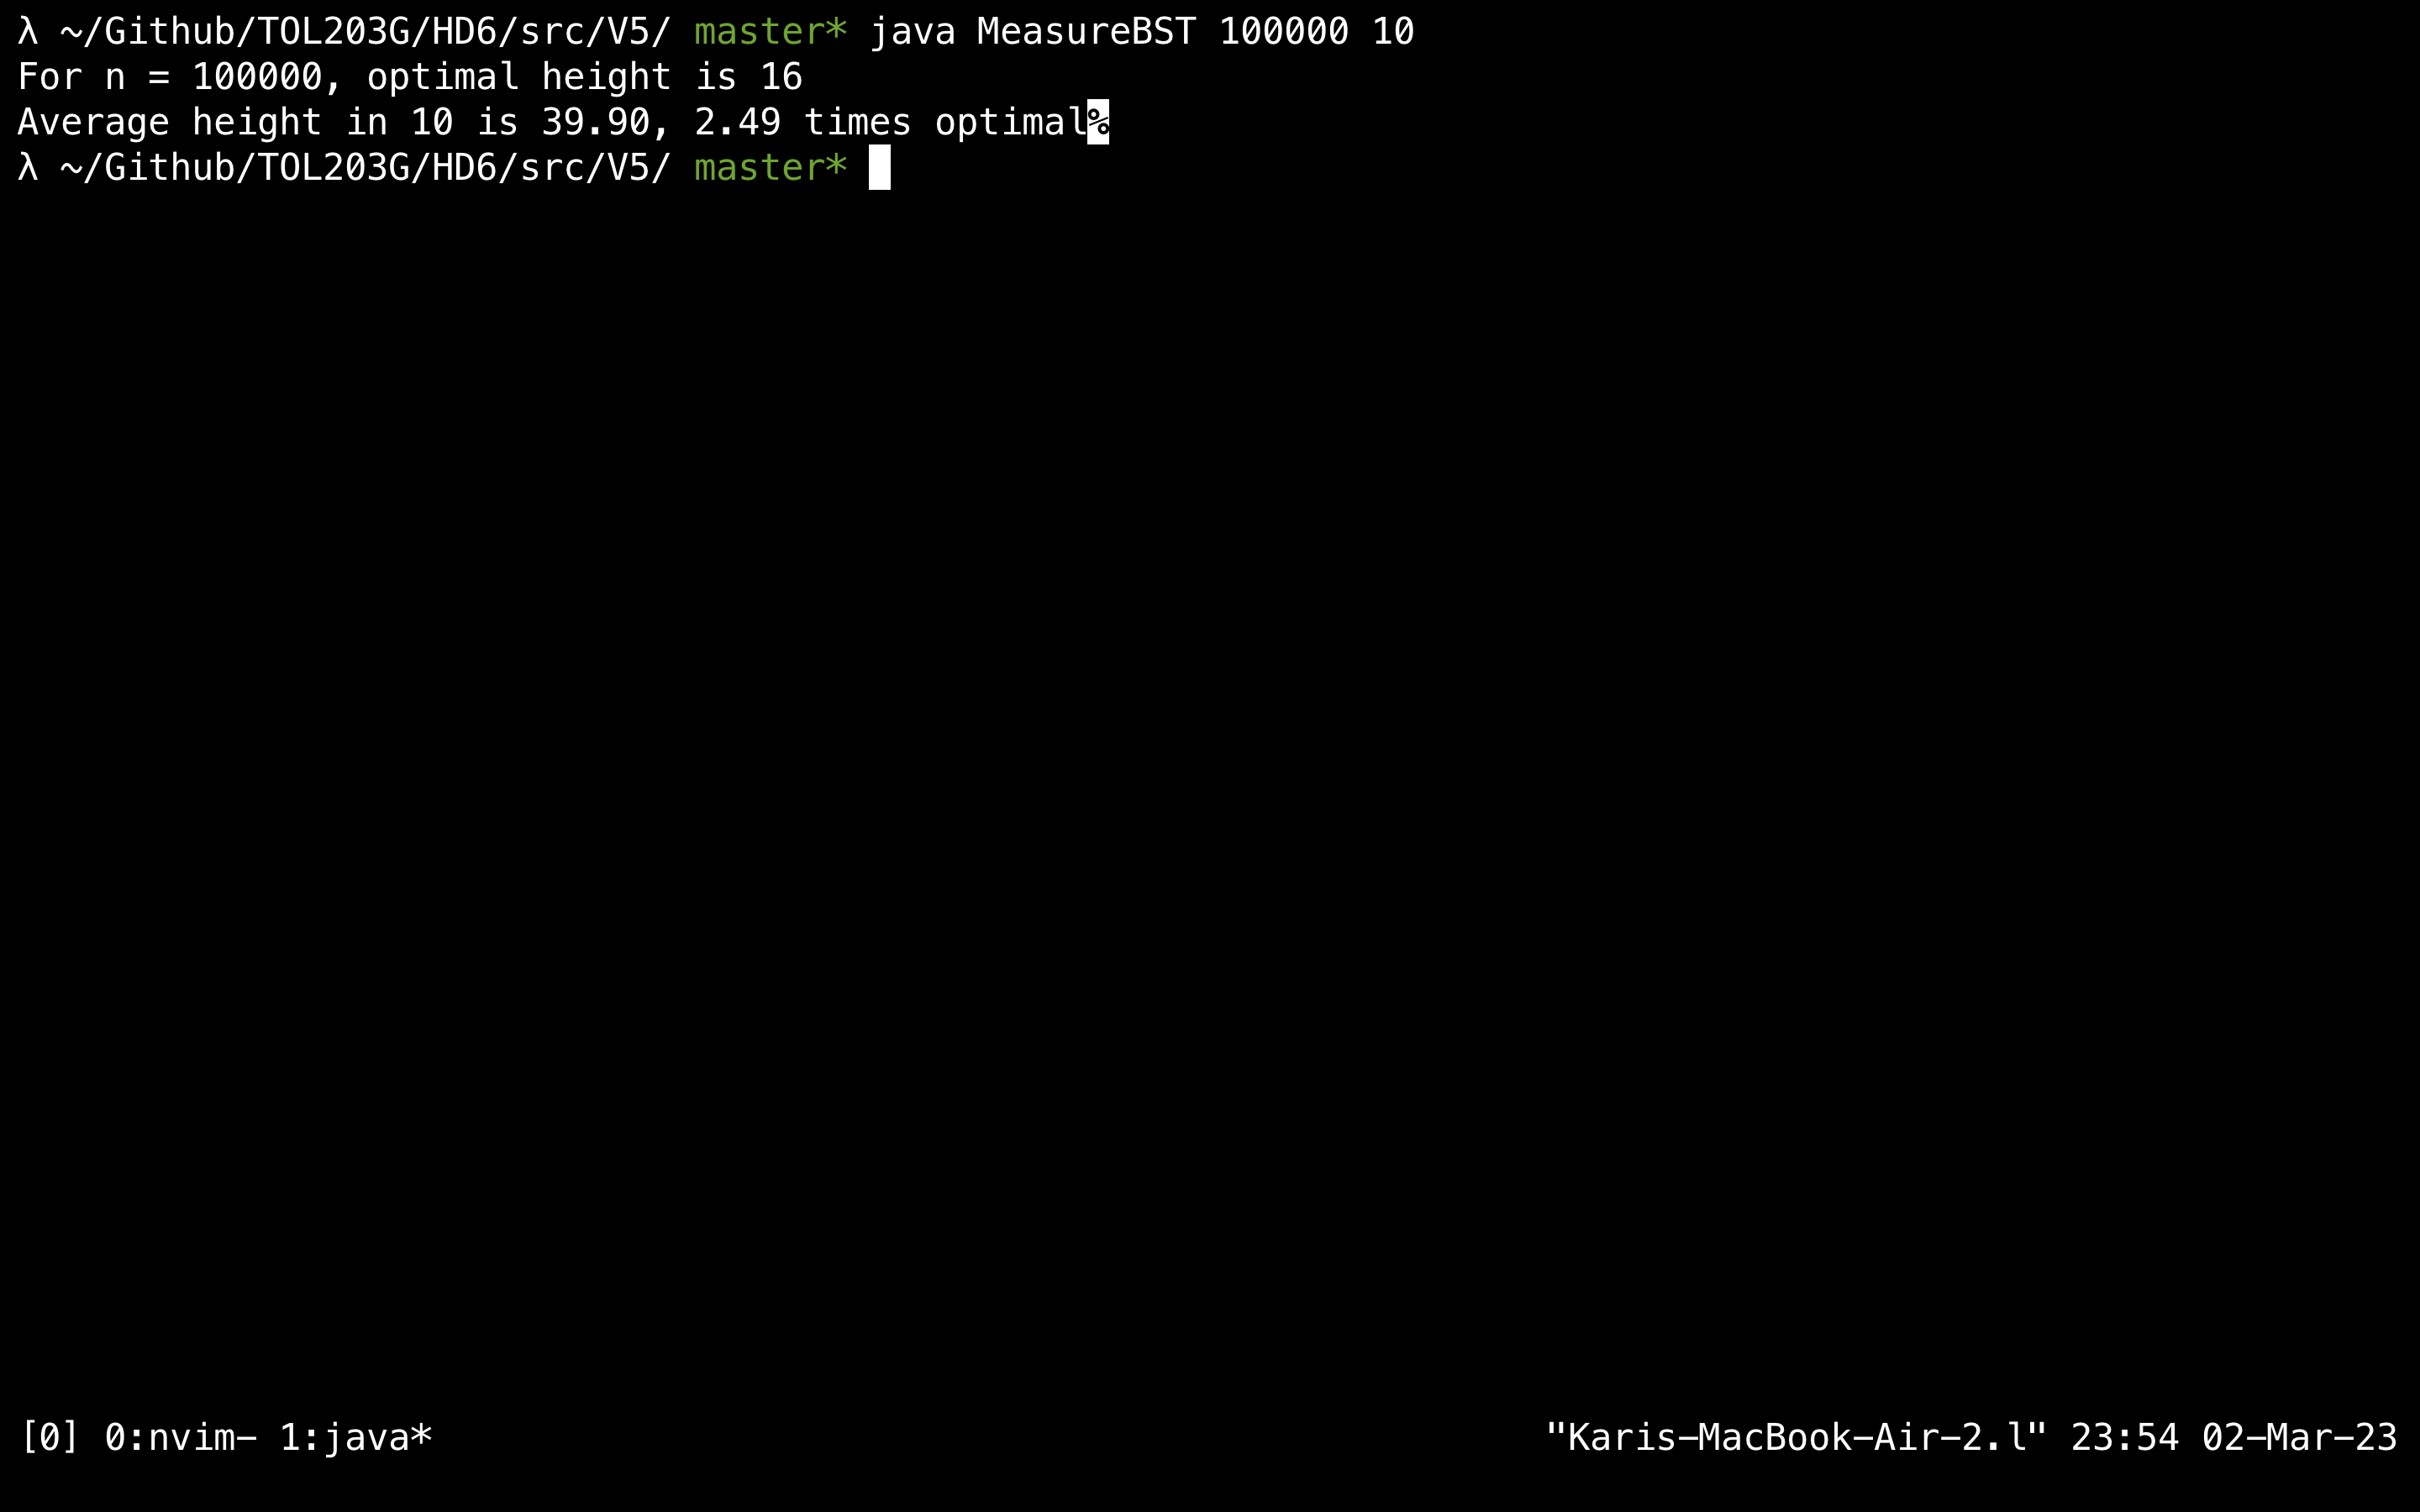
\includegraphics[width=\textwidth]{img/v5-keyrsla.png} 
    \caption{Skjáskot af keyrslu á \texttt{MeasureBST.java}}
  \end{figure}
\end{document}
